
\documentclass[12pt]{article}
\usepackage{amsmath}
\usepackage{amssymb}
\usepackage{amsfonts}
\usepackage{mathrsfs}
\usepackage{bm}
\usepackage{indentfirst}
\setlength{\parindent}{0em}
\usepackage[margin=1in]{geometry}
\usepackage{graphicx}
\usepackage{setspace}
\doublespacing
\usepackage[flushleft]{threeparttable}
\usepackage{booktabs,caption}
\usepackage{float}
\usepackage{graphicx}

\usepackage{import}
\usepackage{xifthen}
\usepackage{pdfpages}
\usepackage{transparent}

\newcommand{\incfig}[1]{%
\def\svgwidth{\columnwidth}
\import{./figures/}{#1.pdf_tex}
}




\title{Econ498 Midterm Summary}
\author{Yan Hao}
\date{Feb 28, 2021}


\begin{document}
\maketitle
\newpage

\section{Program Design}


This program is designed for predicting the criminal type. There are five
steps from data cleaning to model selection.

\subsection{Resize dataset}
Since the raw dataset is quite large, I would like to only focus on criminal
records from 2018 to 2020. The sample data are saved to sample\_data.csv.

\subsection{Draw subset from sample dataset}
There are more than 700,000 observations in sample dataset. There would be 111
columns after I form the dummy variables. Hence, it is necessary to draw a
subset from the sample dataset to simplify the problem. I have drawn 10 percent
of observations to form the subsample, and saved to sub\_sample.csv.

\subsection{Plot criminal type}
I would like to find the pattern of the occurrence for different type of crime.
So I specify each type of crime, and plot their locations with latitude on the
vertical axis and longitude on the horizontal axis. Figure for each criminal
type can be found in figures directory. 

\subsection{Data cleaning}
The program would first drop observations with missing values, extract useful
variables, i.e., Date, Primary Type, Arrest, Domestic, etc. Since Arrest and
Domestic columns are in Bool values, the program converts True and False to
1 and 0. I would like to say that the occurrence of criminal case might 
happen seasonally. Hence, I decompose Date to Month and Hour\_Slot. I would
try to find if particular type of crime would happen during a specific time
period. Moreover, the program convert District, Community Area, and Year 
to dummy variables.

And you can choose to form crime\_count columns by setting count\_crime = True
when you call CleanData. Since each observation belongs to a district, I would 
like to see if the sum of total number of each type of criminal case can improve
the accuracy of the prediction. An example is shown below.

\begin{table}[h!]
\begin{center}
	

\begin{tabular}{cccccc}
\\ [-1.8ex]
\hline
\hline \\[-1.8ex]
{\textbf {Obs}}& {\textbf {District}} & {\textbf {BATTERY}} & {\textbf {CRIMINAL TRESPASS}} & &{\textbf {OTHERS}} \\
\\ [-1.8ex]
\hline \\[-1.8ex]

obs 1 &10.0   &810 	&76		  &...	&0	\\
obs 2 &18.0   &483 	&115		&...	&0	\\
obs 3 &10.0   &810 	&76		  &...	&0	\\
\\ [-1.8ex]
\hline \\[-1.8ex]

\end{tabular}


\end{center}
\end{table}


Observations would have same values in these columns if they belong to same
district, because I assume if the frequency of one type of crime is higher than
others, it would be more likely that the Primary Type of this observation is
this type of crime.

If you set count\_crime = True, the clean dataset will be save to 
CleanData\_with\_crime\_count.csv, otherwise, the dataset would be saved to
CleanData\_without\_crime\_count.csv.


\subsection{Model selection}
Since Primary Type is categorical, RandomForest (RF), Logistic, and SVM can be
used to do the prediction. Same as before, it takes much longer time for 
Logistic and SVM. Hence I do a grid search for RF model. The accuracy rate
for each split is shown in Figure 1 and 2. The accuracy rate decreases while
the maximum depth increases. Also, it seems that the machine works slightly
better with dataset without crime\_count.



\section{Figures}

\begin{figure}[H]
 \caption{Accuracy rate with crime count}
 \center{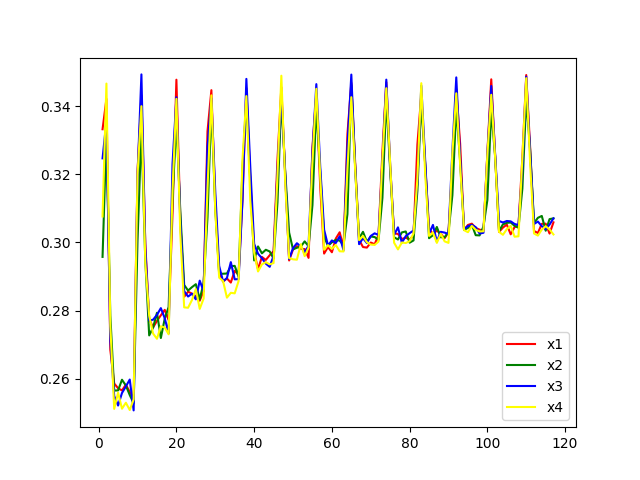
\includegraphics[scale = ]  {figures/acc_trend_RF_with_crime_count.png}}
\end{figure}


\begin{figure}[H]
 \caption{Accuracy rate without crime count}
 \center{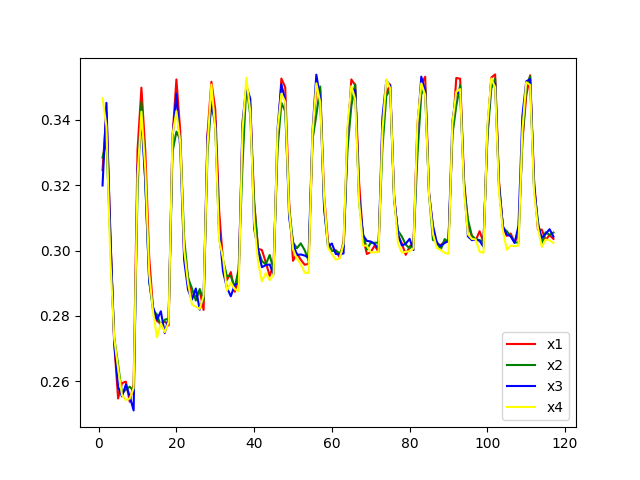
\includegraphics[scale = ]  {figures/acc_trend_RF_without_crime_count.png}}
\end{figure}



















\end{document}

